\documentclass{article}
\usepackage[utf8]{inputenc}
\usepackage{amssymb,amsmath,graphicx,indentfirst}


\title{T1 - Gauss e Cholesky}
\author{George Othon\\NUSP 10349978}
\date{April 2020}

\begin{document}

\maketitle

\section{Introdução}
\par Este relatório tem como finalidade analisar os resultados obtidos para solução de um sistema linear Ax = b a partir dos algoritmos de Eliminação de Gauss (Com e sem pivoteamento) e Fatorização de Cholesky. Assim como, também calcularemos o determinante das matrizes.
\par A análise foi dividida em duas parte, onde na primeira utilizamos a matrix de Hilbert e na segunda um gerador de matrizes aleatórias.
\par Como métrica para a aproximação obtida pela implementação dos algoritmos foi usada a norma 2.

\section{Análise do erro}
Para verificar a proximidade entre o vetor solução x e o vetor aproximado $\hat{x}$ utilizamos a norma euclidiana aprenstada à seguir:
$$
{\displaystyle erro = \|x - \hat{x}\|_{2}={\Big (}\sum _{i=1}^{n}(x_{i} - \hat x_{i} )^2{\Big )}^{\frac {1}{2}}}
$$

\par Com o vetor $b_n$ é composto pela soma da das componentes da linha da matriz de $A_{nxn}$, temos que a solução é $x_i = 1, \ \forall i \in [1,n]$. Sendo assim, quanto mais proximo de zero for o \textbf{erro} melhor a implementação do algoritmo.

\section{Parte I}
Primeiramente, vamos comparar a implemetação da Eliminação de Gauss com pivoteamento e sem pivoteamento, para matrizes de Hilbert.
\newpage

\subsection{Erro}

\par Testamos os dois algoritmos para matrizes quadradas nxn.

%\newpage

\begin{figure}[htb]
    \centering
    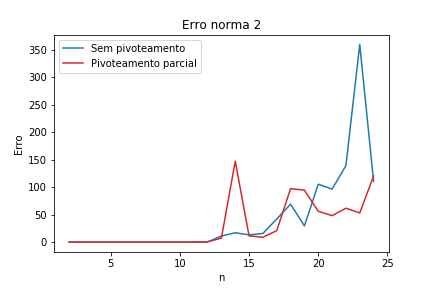
\includegraphics[scale=0.5]{image1.png}
    %\caption{Caption}
    \label{fig:my_label}
\end{figure}

Podemos ver que o erro, para os dois métodos cresce bastante a partir de um certo momento. No pivoteamento parcial temos um outlier um pouco antes de chegar no n = 15, mas após n = 20 ele começa a crescer mais devagar do que no sem pivoteamento.
\par Vamos observar os resultado obtidos até n = 15.

\hfill

\begin{figure}[htb]
    \centering
    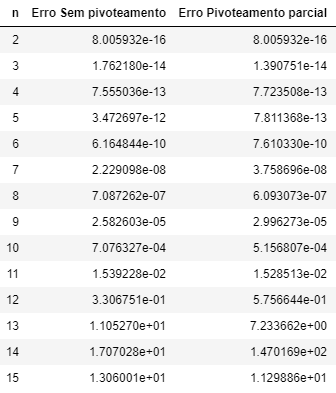
\includegraphics[scale=0.5]{Tabela 1.PNG}
    %\caption{Tabela erro}
    \label{fig:my_label}
\end{figure}

\subsection{Determinante}

\par Para comparar o erro e o valor do determinante foi necessário separar os casos, já que o determento fica muito próximo de zeros nos casos em estudo.
\par Para a eliminação sem pivoteamento:

\newpage

\begin{figure}
    \centering
    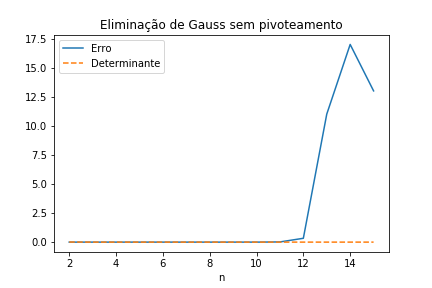
\includegraphics[scale=0.5]{image4.png}
    %\caption{Caption}
    \label{fig:my_label}
\end{figure}

\par E para a eliminação com pivoteamento:
 
 \begin{figure}[ht]
     \centering
     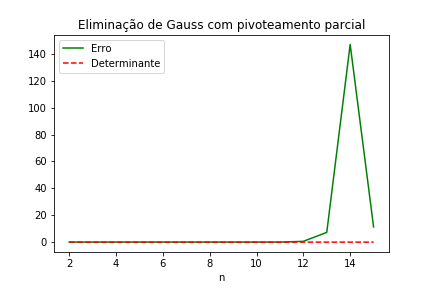
\includegraphics[scale=0.5]{image5.png}
     %\caption{Caption}
     \label{fig:my_label}
 \end{figure}

\par Podemos perceber que até certo ponto, nos dois métodos, o erro fica próximo ao determinante. Para melhor observar foi feita a diferença entre o erro e o determinante.

\begin{figure}[!ht]
    \centering
    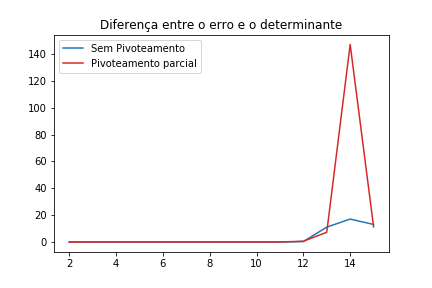
\includegraphics[scale=0.5]{image6.png}
    %\caption{Caption}
    \label{fig:my_label}
\end{figure}

\newpage 

\par Podemos perceber então que até aproximadamente n = 12, o erro fica bastante próximo ao determinante, nos dois casos estudados.


\section{Parte II}
Na segunda parte utilizei um gerador de matrizes $A_{nxn}$ obtida através de uma multiplicação entre uma matrix $M_{nxn}$, onde cada elemento $m_{ij}$ é um número escolhido aleatóriamente do intervalo [-10,10].

\subsection{Erro}

\par Para a decomposição de Cholesky com substiuições direta e reversa obtivemos o seguiinte erro.

\begin{figure}[ht]
    \centering
    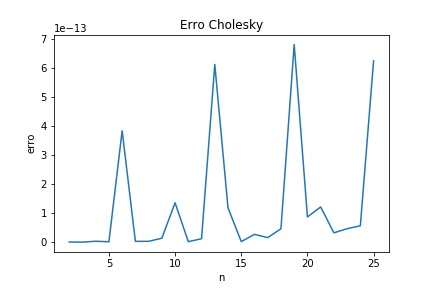
\includegraphics[scale=0.5]{erro_cholesky1.png}
    %\caption{Caption}
    \label{fig:my_label}
\end{figure}

\par Pode-se perceber que o erro varia bastante, mas é sempre próximo á zero, até n = 25 o erro é menor ou igual a $7 x 10^{-13}$.


\par Apesar do crescimento do erro, devido ao maior número de operações para resolver o sistema, o método de Cholesky ainda tem bons resultados para matrizes grandes.

\begin{figure}[ht]
    \centering
    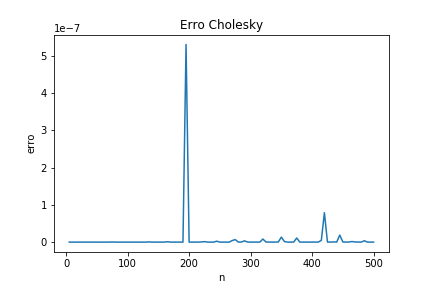
\includegraphics[scale=0.5]{erro_cholesky4.png}
    %\caption{Caption}
    \label{fig:my_label}
\end{figure}

\hfill

\par Quando comparamos os dois algoritmos da Parte I, a implementação de cholesky e a função do numpy temos dificuldade em fazer a análise já que existe uma grande discrepância entre os métodos para a mesma matriz.

\begin{figure}[ht]
    \centering
    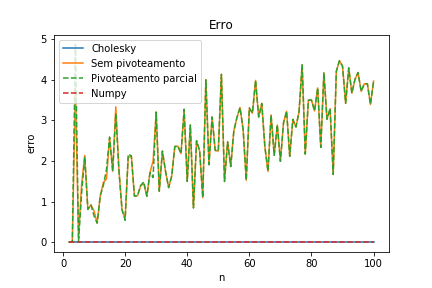
\includegraphics[scale=0.5]{erro_cholesky2.png}
    %\caption{Caption}
    \label{fig:my_label}
\end{figure}

\hfill

Podemos observar um erro muito maior na Eliminação de Gauss, e o método do Numpy e de Cholesky ficam próximo de zero.


\begin{figure}[ht]
    \centering
    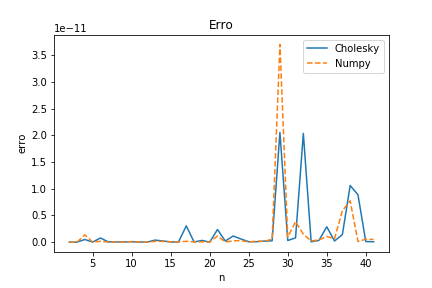
\includegraphics[scale=0.5]{erro_cholesky3.png}
    %\caption{Caption}
    \label{fig:my_label}
\end{figure}

\par Temos então um erro bastante próximo por nossa implementação de Cholesky e o método linagl.solve.

\subsection{Tempo}
Em relação ao tempo, o método de cholesky se apresentou eficiente para n's baixos.

\begin{figure}[ht]
    \centering
    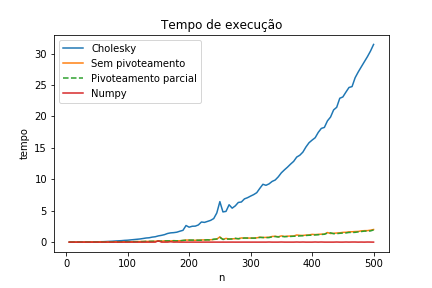
\includegraphics[scale=0.5]{tempo2.png}
    %\caption{Caption}
    \label{fig:my_label}
\end{figure}

Embora o código de Cholesky tenha um crescimento exponecial maior que os outros códigos, ainda se mostra bastante eficaz até aproximadament n = 40, onde fica próximo aos outros métodos.

\subsection{Determinante}

A análise do determinante foi a mais complexa, já que o determinante tem uma variação muito grande com o aumento do n.


\begin{figure}[!ht]
    \centering
    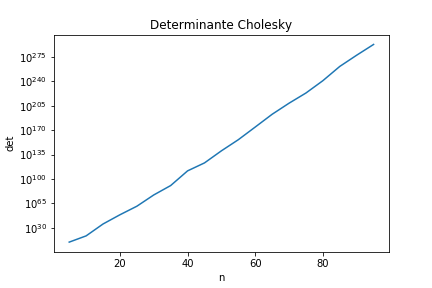
\includegraphics[scale=0.5]{det_cholesky1.png}
    %\caption{Caption}
    \label{fig:my_label}
\end{figure}

Foi utilizado um gráfico com escala logarítmica para analisar o crescimento do determinante. Logo, analisando o gráfico, percebemos uma elevação de forma exponencial.

\hfill

\newpage

\section*{Conclusão}
Com base no que foi apresentado, para as matrizes de Hilbert, o erro foi baixo para valores pequenos de n, fazendo com que os algoritmos de Eliminação funcionassem bem para n até 12. 

\par Tivemos bons resultados com os métodos de Eliminação de Gauss e com a Fatorização de Cholesky nas matrizes geradas aleatóriamente, apontando um erro muito menor para Cholesky do que paras as eliminações de Gauss com e sem pivoteamento. Já ao examinar o tempo computacional, o método de Cholesky tem um crescimento exponencial muito maior que a eliminação. O determinante teve um crescimento exponencial, a escala logarítmica nos ajudou na vizualização da evolução do determinante, onde, nessa escala, nos permite observar uma reta, tornando mais fácil a interpretação da tendência do determinante com o aumento de n.

\par A Fatorização de Cholesky foi o método escolhido como mais eficaz, já que seu erro para n's alto se manteve extremamente próximo de zero, mesmo apresentando um tempo maior, com um crescimento muito mais rápido se mostrou o melhor para resolver sistemas lineares.

\end{document}
